\documentclass[..thesis.tex]{subfiles}

\newtheorem{defin}{Definition}[section]

\begin{document}


\toguide{What is static analysis?}


Under \textit{program analysis} (or just \textit{analysis}) we mean a process of deciding whether some property holds for a program under analysis.
Analysis of a program is \textit{static} if the program being analyzed does not get executed during the analysis, in contrast to \textit{dynamic} analysis,
during what program is executed. Static analysis are often used by compilers, for example for finding uses of variables that are not declared beforehand
in Java or C programs. In addition, modern IDEs constantly run wide selection of static analysis in the background, to enable things such as variable renaming,
for what one would have to know about all the usages of a specific variable in the program, taking into account the relevant scopes. 

\toguide{Why limit ourselves?}


There are good reasons for preferring static analyses over dynamic (or combined) analysis.
To pick a few, it lets us say something about a program that does not compile (and as such, cannot be analyzed dynamically),
it allows to perform our analyses faster compared to dynamic analysis what one cannot perform faster than the time it takes to execute the program
and as static analyses do not depend use any information gathered from a specific run then it is possible to have an analysis that says something
about all the possible runs of a program (and not only, say, for all the possible runs that the analysis has witnessed).
The last reason is, as one can imagine, very helpful in case of data-races. This enables static analysis to output to find that there
 are no errors in the program instead of that it is not able to find any errors -- to verify a program instead of testing it.

\toguide{How is static analysis done?}


As one might guess, there are a lot of techniques that fit the very wide definition given for static analysis. We will be focusing on one of them -- \textit{abstract interpretation}.

\toguide{Okay, what is abstract interpretation?}


To give an intuition on what is abstract interpretation, consider following program:

\begin{lstlisting}[language=C,style=def]
int main(void) {
  int x, y, z;
  x = 0;
  y = -81;
  z = -37
  if (y * z > 0){
    x = 1;
  }
  return x;
}
\end{lstlisting}

One can easily deduce that the program will always exit with error code $1$, without having to calculate the exact value of  $y*z$.
Instead, we can interpret all the values variables have as negative ($-$), $0$ or positive ($+$) and evaluate $y * z$ as $-*- = +$.
This is considerable easier task.

With this simplification, we do lose precision. Lets consider another example:

\begin{lstlisting}[language=C,style=def]
int main(void) {
  int x, y, z;
  x = 0;
  y = -81;
  z = -37;

  if (y * z > 0){
    x = 1;
  }

  if (y * z - y > 0){
    x = 2;
  }
  return x;
}
\end{lstlisting}.


Here, using the interpretation what we successfully applied in previous example, we would not be able to decide the return value of the program. 
When evaluating $y * z - y $, we can rule out any of the possible values. To be able to evaluate product in a similar way previously described,
we could assigns variables set of \textit{possible} values instead. In this case, we would evaluate $y * z - y $ as $\left\lbrace - \right\rbrace * \left\lbrace
- \right\rbrace - \left\lbrace - \right\rbrace = \left\lbrace -,0,+ \right\rbrace$. Although we cannot decide what the program will return,
we can decide based on the analysis, that the first $if$ block can safely be ignored -- an optimization a compiler could perform.

To build a mathematically sturdy foundation for abstract interpretation we first need to give a more formal definition for executing a program.
 For that, lets give a formal definition of a program.

\begin{defin}
Procedure $p$ is a \textit{control flow graph} $\left( N_p,E_p,s_p,r_p \right)$, where $N_p$ is a finite set of nodes, $s_p \in N_p$
 is the \textit{entry} node with in-degree $0$ and  $r_p \in N_p$ is the \textit{return} node with out-degree $0$. Set of labels $L$ consists of
\begin{itemize}
\item statements $s \in Stmt$, other than procedure calls.
\item procedure calls $p()$, where $p \in Exp$ is an expression, 
\item positive and negative guards ( $Pos\left( e \right) in Guards$ and  $Neg \left( e \right) \in Guards$, $e \in Exp$),
\item and thread spawning function $spawn\left( e \right), e \in Exp$.  
\end{itemize}
The edge set  $E_p \subseteq N_p \times L \times N_p$. In addition, we require that out-degree of node $n \in N_p$ is no bigger than $2$ 
and if $e_1$ and $e_2$ are outgoing edges of $n$ and $e_1 \neq e_2$, then one of $e_1$ and $e_2$ is a positive guard and other a negative guard. 
\end{defin}

It is worth mentioning that although we have constrained ourselves with procedure calls without any arguments and only one return node, those issues can be easily solved with use of global variables. 

In addition, we assume that for every $n \in N_p$, there exists a path from $s_p$ to $n$ and from $n$ to $r_p$. \toadd{do I need this?} 

\begin{defin}
Program $P = \left( Proc, main \right)$, where $Proc$ is a finite set of procedures such that for every $p,q \in Proc, p \neq q \implies N_p \cap N_q = \emptyset$ and $main \in Proc$ is one of the procedures designated as the main function. Let $N$ be set of all nodes in the program, that is $N = \bigcup_{p \in Proc}N_p$ and $E$ be a set of all edges in the program, that is $E = \bigcup_{p \in Proc}E_p$. 
\end{defin}


\begin{figure}[H]
  \begin{center}
    \begin{tikzpicture}[node distance=2cm]

      \node (start) [end] {$s_{main}$};
      \node (decl) [node, below of=start] {};

      \node (assign_x) [node,below of=decl] {};
      \node (assign_y) [node,below of=assign_x] {};
      \node (assign_z) [decision,below of=assign_y] {};

      \node (x_assign_1) [node, below right of = assign_z] {};

      \node (if_y_times_z_minus_y) [decision,below left of = x_assign_1] {};
      \node (x_assign_2) [node, below right of = if_y_times_z_minus_y] {};

      \node (after_second_if) [node, below left of = x_assign_2] {};

      \node (end) [end, below of  =  after_second_if] {$r_{main}$};

      \draw [arrow] (start) -- node [anchor=west] {\small{int x, y, z}} (decl);

      \draw [arrow] (decl) -- node [anchor=west] {\small{x = 0}} (assign_x);
      \draw [arrow] (assign_x) -- node [anchor=west] {\small{y = -81}} (assign_y); 
      \draw [arrow] (assign_y) -- node [ anchor=west] {\small{z = -37}} (assign_z);
      
      \draw [arrow] (assign_z) --
        node [ anchor=west] {\small{$Pos$(y $*$ z > 0)}} (x_assign_1);
      \draw [arrow] (x_assign_1) -- node [ anchor=west] {\small{x = 1}} (if_y_times_z_minus_y);

      \draw [arrow] (assign_z) --
        node [ anchor=east] {\small{$Neg$(y $*$ z > 0)}} (if_y_times_z_minus_y);
   
        
      \draw [arrow] (if_y_times_z_minus_y) --
        node [ anchor=west] {\small{$Pos$(y $*$ z  - y > 0)} } (x_assign_2);
      \draw [arrow] (x_assign_2) -- node [ anchor=west] {\small{x = 2}} (after_second_if);

      \draw [arrow] (if_y_times_z_minus_y) --
        node [ anchor=east] {\small{$Neg$(y  $*$ z - y > 0)}} (after_second_if);
      
      \draw [arrow] (after_second_if) -- node [ anchor=west] {\small{return x}} (end);

    \end{tikzpicture}
  \end{center}
  \caption{CFG corresponding to the last code snippet}
\end{figure}

\toask{Should listings be given names? Seems bit too heavyweight to wrap them in figures, but would make citing so much easier}

As it is not feasible to offer a formalization of all the statements and expressions available in any of common higher-level programming languages as a part of this thesis, we have elected to leave the sets $Stmt$ and $Exp$ formally undefined, instead relying on readers previous experience with statements and expressions in any of the C family languages.   For the interested, a formalization of a subset of C is done by Vojdani \todo{Cite to doctoral thesis}.

\toask {very clumsy, but would like to bring this up and not just leave the sets undefined}

\toguide{So, what can we do with this program?}

\toask{Subsectioning?}

Now that we have defined how program looks, we will continue with how such a program is evaluated -- the \textit{semantics} of the program.

From here on we will use following notation to ``update'' a function:

\begin{equation*}
f \left[ x : a \right] \left( y \right) = 
  \begin{cases}
  a & y = x \\
  f \lp  y \rp & otherwise \\ 
  \end{cases}
\end{equation*}.

Lets first consider single threaded programs. Let $S$ be set of states of the program, that is $s : Var \to Val$, where $Var$ is set of variables in the program and $Val$ is set of possible values. Again, we will not formally define sets $Val$ and $Var$ here. For every statement $stmt \in Stmt$, let $ \lllb s \rrrb_{Stmt} : S \to S$ be a function that updates the state of the program. 

For example

\begin{equation*}
 \lllb x = 3 \rrrb_{Stmt} (s) = s \left[ x : 3 \right] \text{.}
\end{equation*}

Similarly, for every expression $e \in Exp$, let $\lllb e \rrrb_{Exp} : S \to Val$ that evaluates expression in context of the state. 

For example, let $s$ be a state after assigning $3$ to $x$, that is

\begin{equation*}
s = \lllb x = 3 \rrrb_{Stmt} (s_0) \text{,}
\end{equation*},
where $s_0$ is an arbitrary state. 

Then 
\begin{equation*}
\lllb x + 8 \rrrb_{Exp} \left( s \right) = 11 \text{.}    
\end{equation*}

With this in mind, we can define a relation for intra-procedural evaluation of our programs as follows:

\begin{defin}
Intra-procedural evaluation relation of procedure $p$, $\intraproc_p \subseteq  \lp N_p  \times S \rp  \times \lp N_p \times S \rp$ is a relation for what following rules hold:

\addtolength{\jot}{2em}
\begin{gather*}
  \inference[Stmt]{ \lp u, stmt, v \rp \in E_{p}  \separ  \lllb stmt \rrrb_{Stmt} \lp s \rp = s'}{\lp u, s \rp \intraproc \lp v, s' \rp} \\
  \inference[Pos]{ \lp u, Pos \lp e \rp , v \rp \in E_{p} \separ \lllb e \rrrb_{Exp} \lp s \rp = true }{\lp u, s \rp \intraproc \lp v, s \rp} \\  
  \inference[Neg]{ \lp u, Neg \lp e \rp , v \rp \in E_{p} \separ \lllb e \rrrb_{Exp} \lp s \rp \neq true }{\lp u, s \rp \intraproc \lp v, s \rp} 
\end{gather*}
\addtolength{\jot}{-2em}

\end{defin}

This relation gives a formal definition for one atomic step during evaluation of a procedure, when evaluating a procedure step with the relation $\intraproc$, the rule applied depends on the type of the edge under evaluation. 

\toguide{ What about procedure calls?}

To support inter-procedural evaluation of our program, we need to keep track of the caller of process. For that we will use, as is usually done, a \textit{call stack}. Call stack is a tuple of CFG nodes, first node is current CFG node (the one being evaluated) and rest of nodes are call sites, points from where program evaluation should continue after reaching the return node. Let $Stack$ be set of all call stacks of program $P$. 

We will define inter-procedural evaluation relation for single-threaded program $P$ as follows:

\begin{defin}

Inter-procedural evaluation relation of single-threaded program $P$, $\interproc \subseteq \lp Stack \times S \rp \times \lp Stack \times S \rp$ is a relation for what following rules hold:

\addtolength{\jot}{2em}
\begin{gather*}
  \inference[Stmt]{\lp u, stmt, v \rp \in E  \separ \exists p \in P  \lp u, s \rp \intraproc_p \lp v, s' \rp }{ \lp u :: xs, s \rp \interproc \lp v :: xs, s` \rp} \\
  \inference[Pos]{ \lp u, Pos \lp e \rp, v \rp \in E \separ   \lllb e \rrrb_{Exp} \lp s \rp = true  }{\lp u :: xs , s \rp \interproc \lp v :: xs, s \rp} \\ 
  \inference[Neg]{ \lp u, Neg \lp e \rp, v \rp  \in E \separ   \lllb e \rrrb_{Exp} \lp s \rp \neq true  }{\lp u :: xs , s \rp \interproc \lp v :: xs, s \rp} \\
  \inference[Call]{ \lp u, p\lp\rp , v \rp  \in E \separ  \lllb p \rrrb_{Exp} \lp s \rp = proc \separ proc \in Proc }{\lp u :: xs , s \rp \interproc \lp s_{proc} :: v :: xs, enter_{proc} s \rp} \\
  \inference[Return] { proc \in Proc} { \lp r_{proc}::xs , s \rp \interproc \lp xs, return_{proc} s \rp}
\end{gather*}
\addtolength{\jot}{-2em}

where $enter_{proc}$ and $return_{proc}$ are state transformers that initialize and destroy local variables.

\end{defin}d 

\toask{What about threads?}

To support multithreaded programs, we will first expand our inter-procedural evaluation relation to support the thread spawning function $spawn$.

\begin{defin}

Intra-thread evaluation relation of $P$, $\intrathread \subseteq  \lp Stack \times S \rp \times \lp Stack \times S \times Proc^\ast \rp$ is a relation for what following rules hold:

\addtolength{\jot}{2em}
\begin{gather*}
  \inference[Spawn]{\lp u, spawn(p), v \rp \in E  \separ  \lllb p \rrrb_{Exp} = proc \separ proc \in Proc  }{ \lp u :: xs, s \rp \intrathread \lp v :: xs, s, (proc) \rp} \\
  \inference[Pos,Neg,Call,Return] {\lp u, stmt, v \rp \in E \separ \lp xs , s \rp \interproc \lp ys, s' \rp }{ \lp xs , s \rp \intrathread \lp ys, s', \lp \rp \rp}
\end{gather*}
\addtolength{\jot}{-2em}

\end{defin}

\toask{ Okay, but the process list is not used anywhere?}

The added information about spawned threads will be used by the following relation.

\begin{defin}

 The inter-thread evaluation relation of $P$, $\interthread \subseteq \lp Stack^\ast \times S \rp \times \lp Stack^\ast \times S \rp$ is a relation for what following rule holds:   

\begin{equation*}
  \inference{ 0 \leq i \leq n  \separ \lp xs , s \rp \intrathread \lp ys, s', \lp p_1^\star, \ldots, p_k^{\star} \rp \rp}{ \lp \lp t_0, \ldots, t_n \rp, s \rp \interthread  \lp \lp t_0, \ldots, t_n, \lp s_{p_1^{\star}} \rp, \ldots, \lp s_{p_k^{\star}} \rp  \rp , s' \rp} \text{.}
\end{equation*}

\end{defin}

In the $\lp \interthread \rp$ relation, the list of stacks corresponds to call stacks of all the threads currently running. It is worth noting that relation $\lp \interthread \rp$ is non-deterministic if there is more than one thread in the program -- a property that multithreaded programs have.

The $\lp \interthread \rp$ lets us define a set of all possible states of a program $P$, with starting state $s_0$ :

\begin{equation*}
\allstates = \left\lbrace  z | \lp \lp s_{main} \rp, s_0 \rp \interthread^{\ast} z \right\rbrace \text{.}
\end{equation*}


\toask{So, what is the point of this?}

Equipped with set \allstates we would have information about the program at any possible execution point. At the same time, it is clear that computing the set \allstates is not feasible in most cases -- the set might not be finite and even if it is, the all possible states of even a simple program might be quite big.

As in the example we gave at the start of this section, we can however simplify the program by \textit{abstracting} away parts of the state that are not interesting for us for finding out if a certain property holds for the program under analyses. However, it is not easy to get the level of abstraction right, as abstracting away too much does not let us tell much about non-trivial properties of the program and abstracting away too little leaves us with task that is too big to feasible compute.

\toask{So, how are we abstracting?}

To have our abstraction on a sound footing, we need a formalization of the idea. The mathematical  theory of \textit{complete lattices} offers a suitable framework. We will now give a short introduction to the lattice theory.

\toask{Okay, lattice theory?}

First of all, a quick reminder from set theory.

\begin{defin}[Partial Order]
A set $D$ with relation $\sqsubseteq \subseteq D \times D$ is called a \textbf{partially ordered set} if $\sqsubseteq$ is a \textbf{partial order}, that is reflexive, antisymmetric and transitive.
\end{defin}

\begin{defin}[Upper bound]
Let $\lp D, \sqsubseteq \rp$ be a partially ordered set. An \textbf{upper bound} of set $X \subseteq D$,  is an element $x \in D$, such that for every element in $y \in X$, $y \sqsubseteq x$. Element $x$ is the \textbf{least upper bound} of set $X$, denoted as $\bigsqcup X$ if for every other upper bound $z$ of $X$, $x \sqsubseteq z$.  
\end{defin}

\begin{defin}[Lower bound]
Let $\lp D, \sqsubseteq \rp$ be a partially ordered set. An \textbf{lower bound} of set $X \subseteq D$  is an element $x \in D$, such that for every element in $y \in X$, $x \sqsubseteq y$. Element $x$ is the \textbf{greatest lower bound} of set $X$, denoted as $\bigsqcap X$ if for every other lower bound $z$ of $X$, $z \sqsubseteq x$.    
\end{defin}

Equipped with these three definitions, we can now define \textit{complete lattice}:

\begin{defin}[Complete lattice]
A tuple $\lp D, \sqsubseteq \rp$ is a complete lattice if $D$ is a partially ordered set with relation $\sqsubseteq$ and for every set $X \subseteq D$, there exists $\bigsqcup X$ and $\bigsqcap X$.
\end{defin}


We will use notation $x \bigsqcup \lp  \bigsqcap \rp y$ to denote $\bigsqcup \lp \bigsqcap \rp \lb x, y \rb$ and $\bot$ to denote the least element in $D$, that is $\bot = \bigsqcap D$ and $\top$ to denote the greatest element in D, $\top = \bigsqcup D$.

\toask{So many definitions, what is this (complete) lattice thing?}

Lets now have a look at couple of examples. 

First of all, let $D$ be $\lb true, false \rb$ and let $\sqsubseteq = \lb \lp false, true \rp \rb$. Then $true = \top = \bigsqcup D$ and $false = \bot = \bigsqcap D$. An usual way to describe lattices is the use of Hasse diagrams, graphs that have as nodes the elements of $D$ and there is an edge between $u, v \in D$ if $u \sqsubseteq v$. The edges that are implied by reflexivity or transitivity are usually omitted.

\begin{figure}[H]
  \begin{center}
    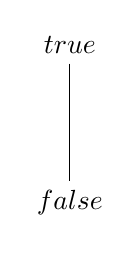
\begin{tikzpicture}
      \node (true) at (0,1) {$true$};
      \node (false) at (0,-1) {$false$};
      \draw (true) -- (false);
    \end{tikzpicture}
  \end{center}
  \caption{$\lp \lb false, true \rb, \lb \lp false, true \rp \rb \rp$ as an Hasse diagram.}
\end{figure}
 
Secondly, to in the example we used to gain intuition about abstract interpertation, we gave each variable a set of its possible values at that program state. Under the values we differianted between negative integers, zero and positive integers. The corresponding lattice would be the following.


\begin{figure}[H]
  \begin{center}
    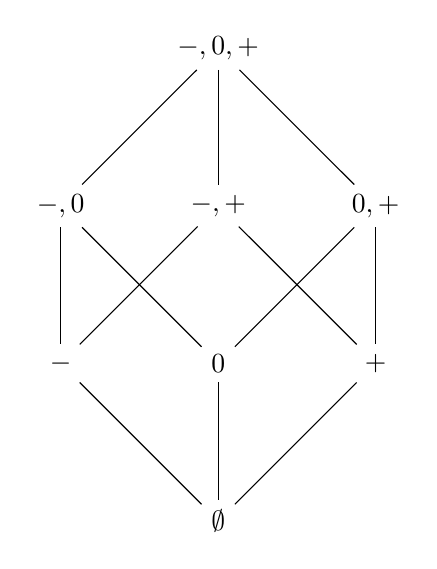
\begin{tikzpicture}
      \node (D) at (0,2) {$\lb -,0,  + \rb$};

      \node (minuszero) at (-2,0) {$\lb -, 0 \rb$};
      \node (minusplus) at (0,0) {$\lb -,+ \rb$};
      \node (zeroplus) at (2,0) {$\lb 0,+ \rb$};

      \node (minus) at (-2,-2) {$\lb - \rb$};
      \node (zero) at (0,-2) {$\lb 0 \rb$};
      \node (plus) at (2,-2) {$\lb + \rb$};

      \node (empty) at (0,-4) {$\emptyset$};

      \draw (D) -- (minuszero);
      \draw (D) -- (minusplus);
      \draw (D) -- (zeroplus);

      \draw (minuszero) -- (minus);
      \draw (minuszero) -- (zero);

      \draw (minusplus) -- (minus);
      \draw (minusplus) -- (plus);

      \draw (zeroplus) -- (zero);
      \draw (zeroplus) -- (plus);

      \draw (minus) -- (empty);
      \draw (zero) -- (empty);
      \draw (plus) -- (empty);
    \end{tikzpicture}
  \end{center}
  \caption{$2^{\lb -, 0, + \rb}$, ordered by inclusion}
\end{figure}

It is worth noting that for every set $S$, its powerset $2^S$ is a complete lattice when ordered by inclusion with union of two sets being the least upper bound and intersection being the greatest lower bound.

As a last example, lets look at \textit{flat lattice} -- a lattice defined on a set $S \cup \lb \bot, \top \rb$, with following ordering $\sqsubseteq = \lb \lp  u,v \rp  | u = \bot \land v \in S \lor  u \in S \land  v = \top \rb$. For a concrete example, let $S$ be $\mathbb{Z}$.

\begin{figure}[H]
  \begin{center}
    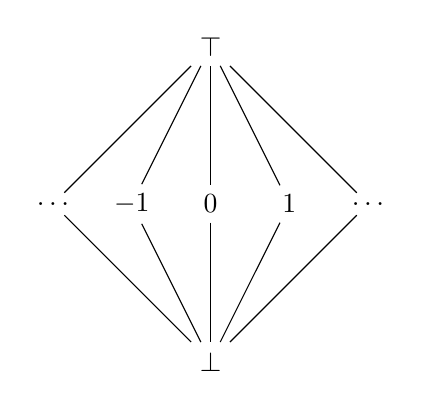
\begin{tikzpicture}
      \node (top) at (0,1) {$\top$};

      \node (neg) at (-2,-1) {$\ldots$}; 
      \node (minus_one) at (-1,-1) { $-1$ };
      \node (zero) at (0,-1) { $0$};
      \node (one) at (1,-1) { $1$ };
      \node (pos) at (2,-1) {$\ldots$}; 

      \node (bot) at (0,-3) {$\bot$};

      \draw (top) -- (neg);
      \draw (top) -- (minus_one);
      \draw (top) -- (zero);
      \draw (top) -- (one);
      \draw (top) -- (pos);

      \draw (neg) -- (bot);
      \draw (minus_one) -- (bot);
      \draw (zero) -- (bot);
      \draw (one) -- (bot);
      \draw (pos) -- (bot);

    \end{tikzpicture}
  \end{center}
  \caption{the flat lattice of $\mathbb{Z}$ }
\end{figure}

The flat lattice is one way to create a complete lattice from any kind of set.

\toask{Okay, but what it has anything to do with abstract interpretation?}

Lattices will serve as \textit{abstract domains} for abstract interpretation.  For our running example, we 

 The idea is to construct the abstract domain  in a way that information about the program is 












  


\textit{abstract domain} --$D$,  a set of states for abstract interpretation. Partially ordered $\left(D,\sqsubseteq \right)$ such that if $n \in N$, $d_1,d_2 \in D$,  $n \in \gamma \left(d_1 \right) $ and $d_1 \sqsubseteq d_2$ then $n \in \gamma \left(d_2 \right)$.


\textit{abstract function} --$\alpha$,  mapping from $N$ to $D$.

\textit{concreitization function} -- $\gamma$, mapping from $D$ to $2^N$.


\textit{context sensitive} -- takes into account the values of parameters of function calls, analyses for each call site vs something that applies for all the call sites.

\textit{complete latice} -- a partially ordered set $\left( D,\sqsubseteq \right)$ is complete lattice if for every $S \subseteq D$ there is a an upper and lower bound and if there exists a greatest and a . We denote uppor bound of set $S$ as $\bigsqcup S $ and lower bound as $\bigsqcap S$. We denote the least element of a lattice ($\bigsqcap D$) as $\bot$ and the greatest element as $\bigsqcup D$ as $\top$. Note that we by $d_1 \bigsqcup d_2$ we mean  $\bigsqcup \left\lbrace d_1, d_2, \right\rbrace $   and by $ d_1 \bigsqcap d_2$ we mean $\bigsqcap \left\lbrace d_1, d_2, \right\rbrace $.

 

\textit{Merge over all paths} -- 



\end{document}